% Updated 2024-11-30 15.52
% source: Climate modeling notes EXPLORING +SST

\chapter{SST Forcing}
One of the primary ways climate forcing impacts SSTs is through changes in radiative energy balance. For instance, increasing greenhouse gas concentrations trap outgoing longwave radiation, causing the Earth’s surface, including the oceans, to warm. Oceans absorb more than 90\% of this excess heat, resulting in widespread SST increases. The effects are not uniform, as ocean dynamics influence regional variations in warming. For example, the Western Pacific Warm Pool retains more heat due to strong stratification, while upwelling regions, such as the eastern Pacific, may experience slower warming due to the cooling effects of vertical mixing and horizontal ocean currents.

Other forms of climate forcing also influence SSTs. Volcanic aerosols and human-emitted sulfate aerosols, for example, reflect incoming solar radiation, leading to localized or even global cooling of SSTs. The cooling effects are often more pronounced in the Northern Hemisphere, where industrial activity has historically been concentrated. In contrast, variations in solar radiation cause more subtle, global SST changes due to the ocean’s high heat capacity.

\paragraph{SST Changes as Feedback to Climate Forcing.}
SST changes resulting from climate forcing do not only respond passively but also act as drivers of feedback mechanisms that amplify or modulate the effects of climate forcing. A key example is the water vapor feedback. Warmer SSTs increase evaporation rates, introducing more water vapor into the atmosphere. Since water vapor is a potent greenhouse gas, this enhances warming further. Similarly, SST changes influence cloud formation, which can either reflect sunlight back to space (cooling the Earth) or trap outgoing heat (warming the Earth). The balance of these cloud feedbacks is a significant area of ongoing research.


SST changes driven by climate forcing also amplify or modify major climate phenomena. One well-known example is the El Niño-Southern Oscillation (ENSO). Global warming is thought to alter SST patterns in the tropical Pacific, potentially affecting the frequency or intensity of El Niño and La Niña events. For instance, by flattening the SST gradient between the eastern and western Pacific, warming may weaken the Walker Circulation and favor more frequent El Niño-like conditions. Such shifts have significant implications for global rainfall patterns, droughts, and extreme weather events.

Changes in SSTs also influence large-scale ocean circulation patterns, such as the Atlantic Meridional Overturning Circulation (AMOC). Climate forcing that warms SSTs in the North Atlantic can disrupt this critical current system, leading to cascading effects on regional climates, including shifts in monsoons and weather systems across Europe and North America.

Long-term observations provide clear evidence of the impact of climate forcing on SSTs. Since the late 19th century, global SSTs have risen by approximately 0.8°C, primarily driven by greenhouse gas emissions. However, the warming is not evenly distributed. For example, the Arctic Ocean has experienced significantly faster warming due to the ice-albedo feedback, where melting ice exposes darker ocean surfaces that absorb more solar energy. Meanwhile, regions with persistent upwelling, such as the coast of Peru, have shown slower warming because cooler waters are constantly brought to the surface from the deep ocean.


From greenhouse gases, aerosols, or volcanic activity—can alter the strength and structure of the Walker Circulation by modifying the SST patterns or atmospheric stability.
ENSO Events (a result of internal variability but influenced by external forcing): El Niño events weaken the Walker Circulation as warm SST anomalies dominate the central and eastern Pacific; La Niña events strengthen it as cooler SSTs enhance upwelling in the east and convection in the west.
Observational studies found the importance of SST in the forcing of atmospheric anomalies.


\section{How can surface sea temperature impact atmospheric circulation?}

Let's consider the vorticity equation
\begin{equation}\label{eq. 2.1}
	\frac{\partial \zeta}{\partial t} = - \nabla \cdot (\zeta + f) \mathbf{V} = - (\zeta + f) \nabla \cdot \mathbf{V} - \mathbf{V} \cdot \nabla (\zeta + f) = - (\zeta + f) D - \mathbf{V} \cdot \nabla (\zeta + f)
\end{equation}

In equation \ref{eq. 2.1} D is the divergence and it is equal to
\begin{equation}
	D=u_x + v_y = w_z = \frac{\partial w}{\partial z}
\end{equation}

where $\frac{\partial w}{\partial z}$ is the vertical derivative of the vertical velocity and the last term of \ref{eq. 2.1} is the advection.

If we linearize \ref{eq. 2.1}, all the nonlinear terms will be thrown away so that
\begin{equation}\label{eq 2.3}
	\frac{\partial \zeta}{\partial t} = - f D - v \frac{\partial f}{\partial y} = - f D - \beta v
\end{equation}
\begin{equation}
	\frac{\partial \zeta}{\partial t} = - f \frac{\partial w}{\partial z} - \beta v
\end{equation}

The equation \ref{eq 2.3} stresses that vorticity evolves due to these two terms.
Assuming steady motion, meaning vertical derivative of vertical velocity bust be balanced by the advection

\begin{equation}
	f \frac{\partial w}{\partial z} = \beta v
\end{equation}
If I integrate top - bottom this equation, I'll obtain
What about the atmosphere?
\begin{equation}
	\beta V = f(w_{\text{top}} - w_{\text{bottom}})

\end{equation}
where V is the vertical average of v.
This shows that meridional motion must be balanced by vertical velocity if you are in a steady state.
In the atmosphere we need to use a shallow water equation centered at the equation, this means in beta plane approximation.
\begin{equation}
	u_z- fv = -g \frac{\partial u}{\partial x}
\end{equation}

\begin{equation}
	v_z + fu = -g \frac{\partial u}{\partial y}
\end{equation}

So that
$$-\beta_y v = -g \frac{\partial h}{\partial x} + \frac{X}{\rho H}$$
$$\beta_y u = -g \frac{\partial h}{\partial y} + \frac{Y}{\rho H}$$
$$c^2 (u_x + v_y) = -\frac{gE}{\rho}$$
where X, Y, and E are external forcing terms.
These equations are not in balance because I need to add dissipation representing the effects of nonlinear terms.
\begin{equation}\label{eq 2.8}
	r u - \beta_y v = -g \frac{\partial h}{\partial x} + \frac{\rho H}{X}
\end{equation}


\begin{equation}\label{eq 2.9}
	r v +\beta_y u = -g \frac{\partial h}{\partial y} + \frac{Y}{\rho H}
\end{equation}

\begin{equation}\label{eq 2.10}
	r g h + c^2 (u_x + v_y) = -\frac{gE}{\rho}
\end{equation}



These equations \ref{eq 2.8}, \ref{eq 2.9}, \ref{eq 2.10} can be reduced in this form
\begin{equation}\label{2.11}
	\frac{r}{c^2} \left( r^2 + f^2 \right) v - r \left( \frac{\partial^2 v}{\partial x^2} + \frac{\partial^2 v}{\partial y^2} \right) - \beta \frac{\partial v}{\partial x}
	= \frac{1}{\rho H} \frac{r}{c^2} \left( rY - fX \right) + r \frac{\partial E}{\partial y} - \frac{\partial}{\partial x} \left( \frac{\partial Y}{\partial x} - \frac{\partial X}{\partial y} + fE \right)
\end{equation}

If we assume zonally independent motions that are no dependent from x \ref{2.11} becomes
\begin{equation}
	\frac{r^2 + f^2}{c^2} v - \frac{\partial^2 v}{\partial y^2} = \frac{1}{\rho H} \left( \frac{\partial E}{\partial y} - \frac{fX}{c^2} + \frac{rY}{c^2} \right)
\end{equation}
We could solve this equation by eliminating momentum forcing (X,Y)=0 and considering the heating located at a special latitude away from the equator.\\[0.5 cm]

What is the response of the atmosphere?
The bottom panel of Figure \ref{fig: fig2.1} is the upper flow: the stationary response is asymmetric in longitude, and two kinds of equatorial waves (Kelvin and Rossby) develop. Because of this asymmetry, their shapes are different.
Contour lines give the pressure pattern and you're creating two cyclones north and south.
\begin{figure}[h!]
	\centering
	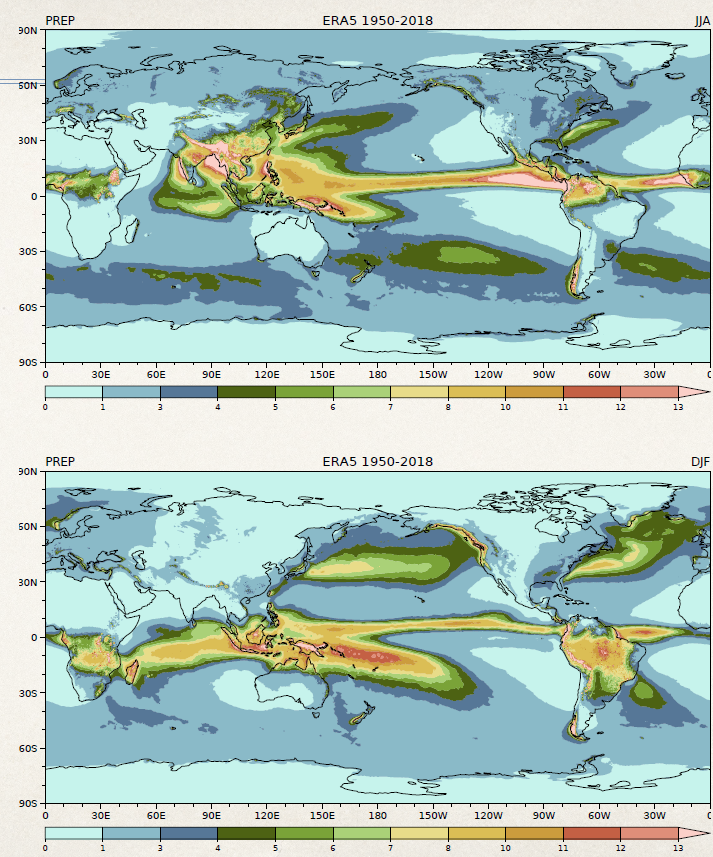
\includegraphics[width=0.5\linewidth]{uploads/24image.png}
	\caption{Enter Caption}
	\label{fig: fig2.1}
\end{figure}

Look that we didn't put any forcing in the equations above, but the heating is creating vortices both in the low and upper levels, which will have consequences. The heating is centered a little bit off the equator but the cyclones are shifted in a more. So the dynamics is that there is a motion due to the heating, but because of the dynamic compensation between divergence and vorticity, in the upper level divergence is compensated by the creation of this cycles.

\begin{figure}[h!]
	\centering
	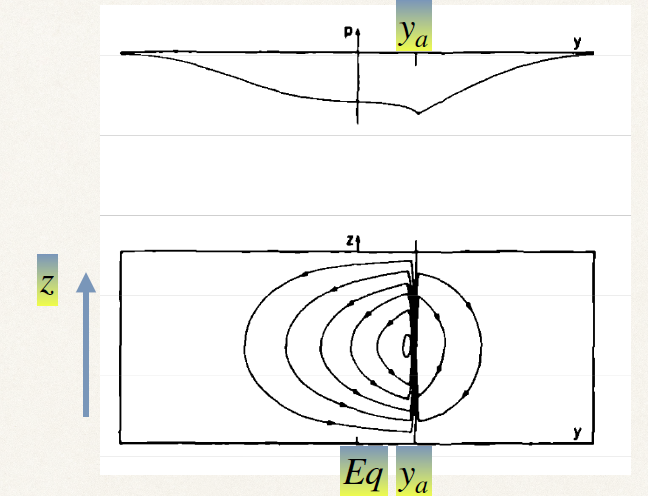
\includegraphics[width=0.5\linewidth]{uploads/23image.png}
	\caption{Enter Caption}
	\label{fig: fig 2}
\end{figure}


As you can see from Figure \ref{fig: fig 2}, the arrows are getting into the heating region, because the air is rising there.
So the pattern is: here there is heating. air is coming into the heating region, goes up, and then goes out. It's not a simple pattern due to the presence of cyclones.
This famous paper shows for the first time, the fact that stationary heating sources provide a stationary response that has a very large scale

However interesting things happen when the heating varies in x, and it is localized as the observation of precipitation shows.
\begin{figure}[h!]
	\centering
	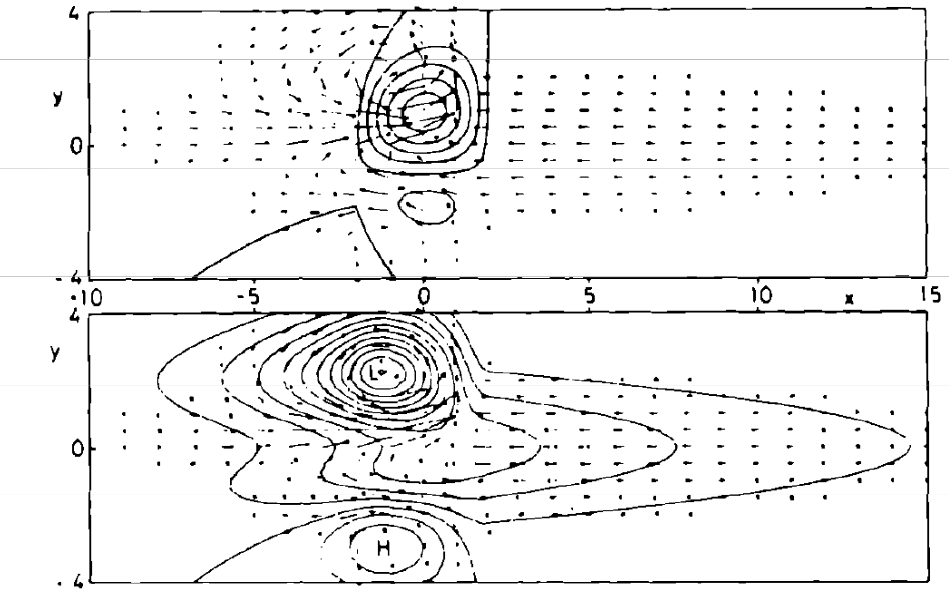
\includegraphics[width=0.5\linewidth]{uploads/25image.png}
	\caption{Enter Caption}
	\label{fig:enter-label}
\end{figure}
\\

An idealized case can be given by
\begin{figure}[h!]
	\centering
	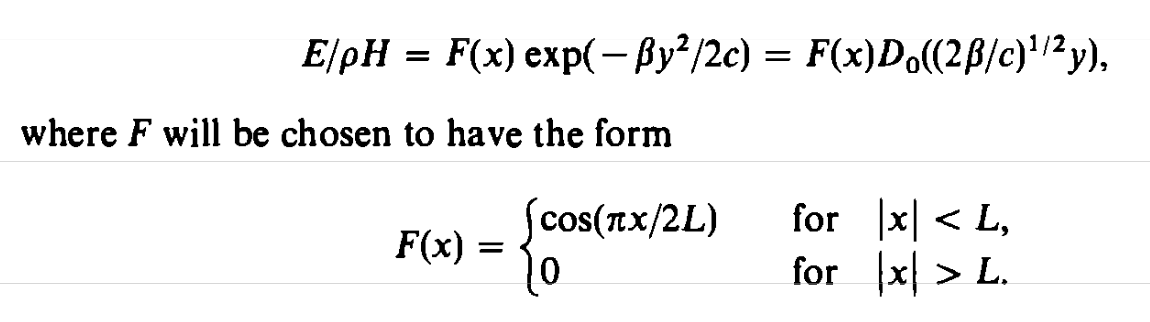
\includegraphics[width=0.5\linewidth]{uploads/22image.png}
	\label{fig:enter-label}
\end{figure}




\\What about if I assume a basic state, meaning a rest atmosphere, and do the same operations as before? Imposing specific boundary conditions led us to a kinematic condition telling us that if air is heating a mountain, this air does not go inside the mountain but the flow will go above it. This phenomenon stresses that mountains are a steady source of vorticity.

If we think at steady motions in the atmosphere there are two main places where you can find
\begin{itemize}
	\item steady heating (equator)
	\item response to the forcing of vorticity of the mountain (mid latitude)
\end{itemize}

In 1979 Grose and Hoskins published a paper describing an investigation that has been conducted of the steady response to orography as described by the linearized shallow-water equations on the sphere.
Results have been obtained for both idealized and realistic climatological mean zonal flows when perturbed by simple isolated mountains.

\begin{figure}[h!]
	\centering
	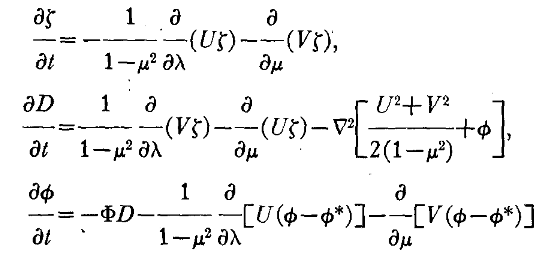
\includegraphics[width=0.5\linewidth]{uploads/19image.png}
	\caption{Equations on the sphere}
	\label{fig: fig 2.2}

\end{figure}
where $\zeta$ is the absolute vorticity, D the divergence, $\Phi$
the average height of the fluid multiplied by the gravitational constant g, $\varphi$ the deviation of the free surface from that height multiplied by g and $\varphi^*$ the height of the orography multiplied by g. The latitude and longitude are denoted by $\theta$ and $\lambda$ with $\mu = \sin \theta$. The variables U and V are respectively the zonal and the meridional velocities multiplied by $\cos \theta$.


The two scientists want to transform equations in Figure \ref{fig: fig 2.2}  in a steady state, to have it they need forcing (external from the system and not described dynamically) and they have to eliminate the time derivative substituting it with the dissipative term.
In particular, the forcing here is represented by $\varphi^*$ because scientists arbitrarily impose it.
They use spectral models to solve shallow water equations, the orography $\varphi^*$ had to be expressed in spherical harmonics and if you do that you'll start to have Gibbs oscillations (Figure \ref{fig:fig 2.5})
Because of the spherical harmonics you get Gibbs waves in both meridional and zonal directions, that is particular evident in South America.
\begin{figure}[h!]
	\centering
	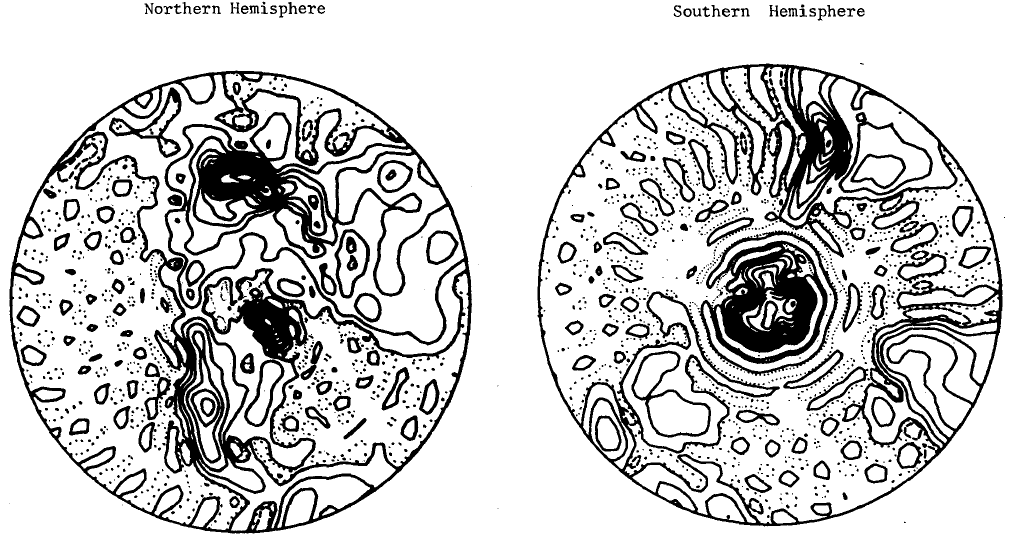
\includegraphics[width=0.5\linewidth]{uploads/26image.png}
	\caption{model earth orography shown in polar stereographic projections}
	\label{fig:fig 2.5}
\end{figure}


\subsection{What is the mechanism by which SST is affecting climate?}

Sea Surface Temperature (SST) plays a critical role in shaping long-term climate variability, particularly on timescales beyond weeks (synoptic timescales), where its influence on atmospheric circulation becomes pronounced. Unlike land surfaces, which adjust quickly to temperature changes and lack long-term memory, the ocean's thermal inertia allows SST to maintain a prolonged impact on the climate system (the rate of change of $T$ is the resulting balance of heat emission). On land, soil moisture provides a limited form of memory, influencing land-atmosphere interactions for up to a year, but the ocean’s capacity to modulate heat exchange and atmospheric patterns makes its effect far more persistent and complex.

The mechanism by which SST affects the atmosphere primarily involves vorticity balance, a key dynamic in atmospheric motion. In equatorial regions, SST anomalies act as localized heating sources, driving convection that alters circulation patterns. When heating occurs, air rises, leading to asymmetrical atmospheric responses in the east-west direction. This localized heating produces cyclonic activity in the lower atmosphere and upper-level vortices displaced from the heating source due to atmospheric dynamics. Localized heating from SST causes air to rise, which in turn generates cyclonic and anticyclonic vortices at different atmospheric levels.  These processes demonstrate how SST anomalies force changes in atmospheric circulation, influencing phenomena such as tropical cyclones, monsoons, and large-scale weather patterns.

\begin{figure}[htp!]
	\centering
	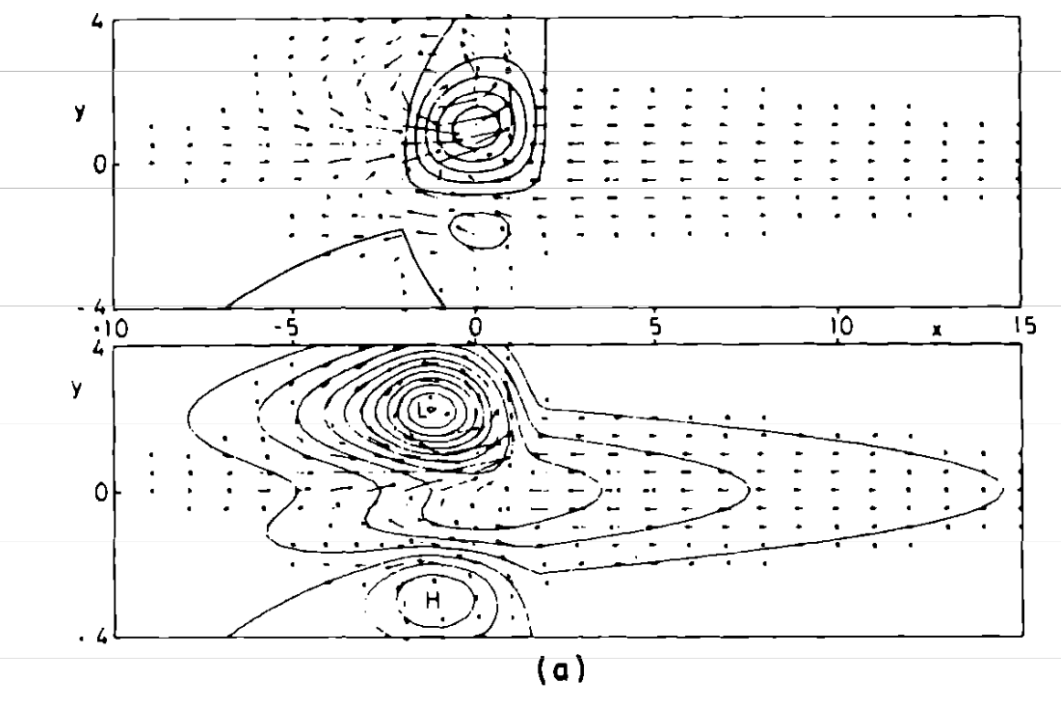
\includegraphics[width=0.4\linewidth]{uploads/Screenshot 2024-11-26 100719.png}
	\caption{Schematic of atmospheric circulation that exhibits cyclonic asymmetry.}
	\label{fig:enter-label}
\end{figure}



In the figure above, the contours represent streamlines or geopotential height isolines in the upper atmosphere, while vectors show wind flow pattern. The cyclonic circulation (low-pressure system "$L$") indicates counterclockwise motion in the NH. The pattern is asymmetrical meaning that the cyclonic core does not produce perfeclty concentric circulation due to asymmetries in forcing. In the high-pressure region "$H$", the arrows and contours suggest a wave-like structure extending downstream of the low-pressure system, representing possibly Rossby waves generated by heating or perturbation. Note that the generation of vorticity in the lower and upper layers may have opposite signs.



In simplified models of atmospheric circulation, such as a barotropic system with constant wind and dissipation, external forcing like heating or topography alters the basic state. Dissipation, including radiative cooling, ensures that the energy added to the system by these forcings does not lead to instability, allowing for a stationary solution. Remember Grose and Hoskins illustrate how mountains can generate Rossby waves, which are planetary-scale atmospheric waves that propagate and redistribute energy and momentum. These waves, influenced by both topographic features and SST anomalies, play a significant role in driving global circulation patterns, such as the jet stream and climate anomalies.

The adjustment to forcing is more challenging over oceans than land because of the ocean’s slower response time. SST anomalies serve as a sustained forcing mechanism, particularly in tropical regions, driving long-term changes in atmospheric circulation through convection and vorticity dynamics. By generating Rossby waves and other large-scale atmospheric responses, SST anomalies influence both local weather events and global climate patterns. This intricate coupling between ocean and atmosphere underscores the importance of SST in understanding and predicting long-term climate variability.\\[0.25 cm]

\subsection{Steady heating balances}
\textbf{Hoskins and Karoly}\cite{Hos81} (1981) investigated the atmospheric response to stationary heating using a General Circulation Model (GCM) with a realistic structure. Their approach involved simplifying a complex mathematical system by linearizing the model. The focus was on understanding the stationary solutions that arise from this linearized problem.

To explore the response to heating, they used discretization methods. This involves breaking down the atmosphere into grid points or using spectral resolution. For example, with a grid resolution of 2 degrees, there are approximately 18000 points (calculated as $180/2×360/2$), and if the model has 9 vertical levels ($\rightarrow$ Manabe), this results in 162,000 unknowns. Solving such a system requires constructing a matrix $\mathbf{A}$, with dimensions based on the degrees of freedom, and then solving the linear equation $\mathbf{A}\mathbf{x}=\mathbf{f}$, where
$\mathbf{x}$ represents the variables of interest, and $\mathbf{f}$ is the forcing vector.

However, directly constructing and solving such a massive matrix is computationally intensive. An alternative approach is to use the model itself, where the prognostic equations are represented as $\mathbf{\dot{x}}=\mathbf{F(x)}$. Adding a heating term $Q$, this becomes $\mathbf{\dot{x}=F(x)}+Q$, since $\mathbf{F(x)}$ is nonlinear, linearization is required to solve for perturbations. By introducing a small perturbation $\mathbf{x'}$ at one grid point: $\mathbf{x=\overline{x}+x'}$, where $\mathbf{x'}$  is structured as a special vector (e.g., $[1,0,0,\dots]$, the model’s response provides the derivative of $\mathbf{F}$ that is just the basic state $\mathbf{\dot{x}=\dot{\overline{x}}}$, forming a i-column of $\mathbf{A}$, corresponding to the position of $1$ in the special perturbation vector. Repeating this process for all degrees of freedom (grid points or spectral coefficients of divergence, vorticity, ... depending on which discretization model you use) constructs the entire matrix.

\paragraph{Balancing heating and advection.}
Let's look at the balances in the thermodynamical equation.
\begin{align}
	\overline{u}\frac{\partial\theta}{\partial x}+{v}\frac{\partial\overline{\theta}}{\partial y}+w\frac{\partial\overline{\theta}}{\partial z}=Q \\
	f\overline{u}\frac{\partial v}{\partial x}-f{v}\frac{\partial\overline{u}}{\partial z}+wN^2=Q
\end{align}
means:
\begin{figure}[htp!]
	\centering
	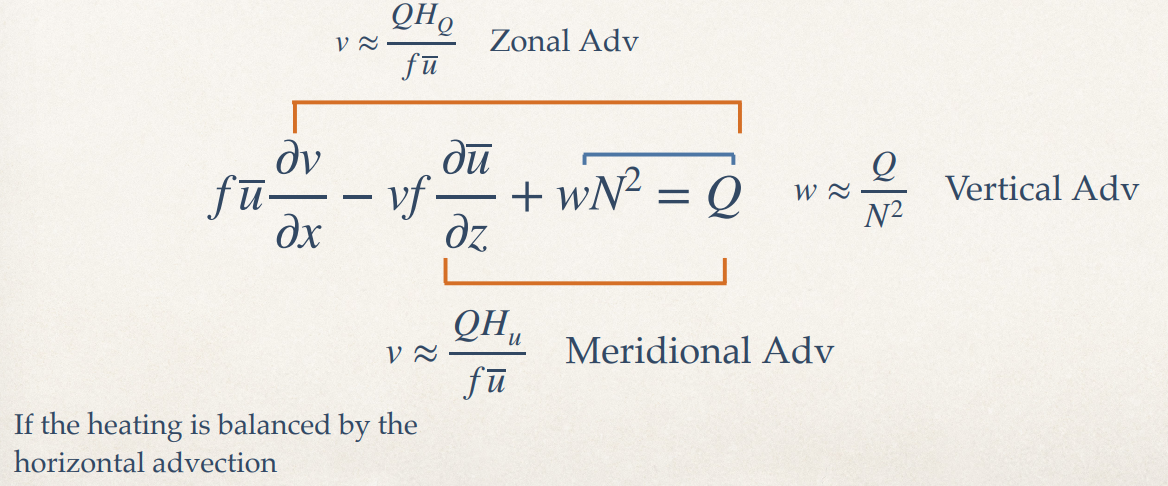
\includegraphics[width=0.5\linewidth]{uploads/Screenshot 2024-11-26 104817.png}
	\caption{heat balance}
	\label{fig:enter-label}
\end{figure}

In the vertical advection case then the vorticity balance is between the beta terms and the stretching term:
$$\beta v\approx fx_z=\frac{fQ}{N^2H_Q}$$
The mechanism with smaller v will dominate, the horizontal advection are of the form:
$$v\approx\frac{QH}{f\overline{u}}$$
and the vertical:
$$v\approx\frac{Q}{N^2}$$
so the dominant process is given by
\begin{equation}
	\gamma=\frac{f\overline{u}^2}{\beta N^2HH_Q}
\end{equation}
Horizontal advection will dominate for small $H_Q$, vertical
advection otherwise. Depending of the size of $\gamma$ heating will balanced by horizontal advection if $\gamma \gg 1$ and by vertical advection if $\gamma\ll 1$.
In the tropics $\gamma$ is small if $H_Q$ is greater than 1 km, so any heating near the surface will generate large meridional motions, but heating away from the surface will generate vertical motions.
\begin{figure}[htp!]
	\centering
	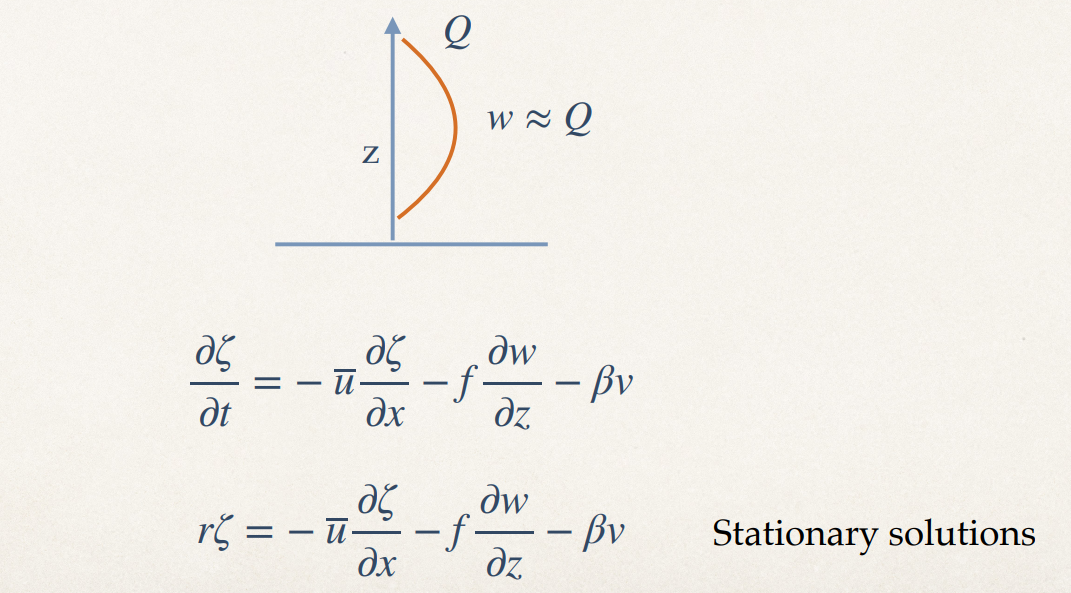
\includegraphics[width=0.5\linewidth]{uploads/Screenshot 2024-11-26 105240.png}
	\caption{Heating and vertical motion}
	\label{fig:enter-label}
\end{figure}


The heating induced by processes like deep convection leads to vertical or horizontal advection, but the dominant mechanism depends on factors such as the stratification of the atmosphere and the strength of the Coriolis parameter. The competition between vertical and horizontal advection can be quantified by a parameter $\gamma$, which helps determine which process dominates, the mechanism generating the smaller advection will dominate as it's easier to treat. In equatorial regions, where SST exceeds 28.5°C, strong deep convection generates significant vertical motion, impacting the overall circulation.

\paragraph{Vorticity balances and responses to heating.}
Heating anomalies, such as those driven by SST, lead to vorticity generation with distinct impacts depending on the region. In the tropics, heating often induces vertical motion and deep convection, while in extratropical regions like the North Atlantic, the vorticity balance is more complex due to baroclinic and barotropic processes. Heating anomalies result in opposite vorticity generation in upper and lower layers, with vertical stratification and horizontal advection playing critical roles.

The implications of anomalous heating differ significantly between regions. For instance, in the North Atlantic, heating anomalies can produce teleconnections, altering large-scale circulation patterns over several months. These teleconnections, resembling the findings of Horace and Wallace on SST variability, highlight how localized heating can influence global atmospheric dynamics.
\begin{figure}[htp!]
	\centering
	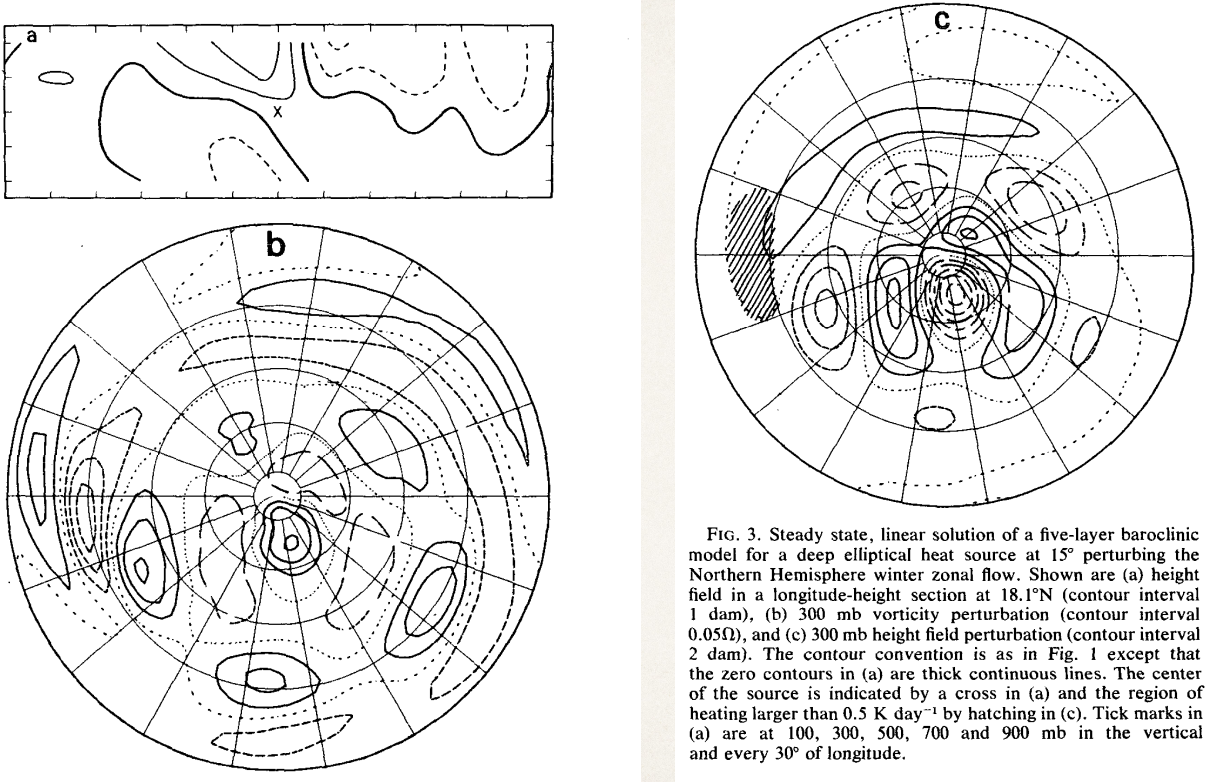
\includegraphics[width=0.4\linewidth]{uploads/Screenshot 2024-11-26 104358.png}
	\caption{steady-state, linear solution of a five-layer baroclinic model.}
	\label{fig:enter-label}
\end{figure}

Teleconnections, or long-distance climate influences, can arise from dynamical causes over intermediate timescales (e.g., months). They are often linked to SST variability and heating-induced circulation changes. However, the assumption of a simple atmospheric basic state limits these analyses because real-world atmospheric states are far more complex.

Atmospheric anomalies tend to grow along gradients, where temperature or pressure contrasts enhance the instability and amplify the response to heating. This gradient-based growth underpins many of the patterns observed in teleconnections and regional responses to SST anomalies.